Jungtinių Amerikos Valstijų bendras vidaus produktas\cite{gdp} 1987 - 2014 metais ir
Jungtinių Amerikos Valstijų gimstamumas\cite{births} tuo pačiu laikotarpiu.
Gimstamumo per mėnesį duomenys buvo akumuliuoti į metinius.

\begin{figure}
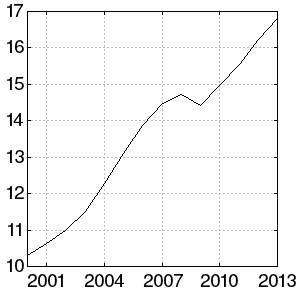
\includegraphics[scale=0.65]{../scripts/gdp_births/gdp.png}
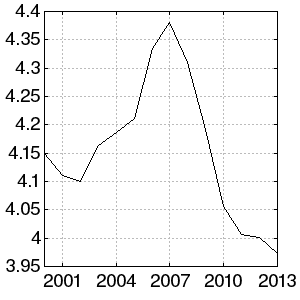
\includegraphics[scale=0.65]{../scripts/gdp_births/births.png}
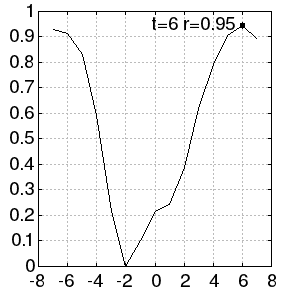
\includegraphics[scale=0.65]{../scripts/gdp_births/result.png}
    \caption{Grafikas kairėje: JAV BVP (trln. USD). Grafikas centre: naujagimių skaičius per metus (milijonais). Grafikas dešinėje: signalų tarpusavio koreliacija}
\end{figure}

Signalų tarpusavio koreliacijos grafikas rodo stiprių ryšį kai \( R_{fg}(t) = 0.95 \) ir \( t = 6 \).

